\documentclass[11pt,a4paper]{article}
\usepackage[spanish,es-nodecimaldot]{babel}	% Utilizar español
\usepackage[utf8]{inputenc}					% Caracteres UTF-8
\usepackage{graphicx}						% Imagenes
\usepackage[hidelinks]{hyperref}			% Poner enlaces sin marcarlos en rojo
\usepackage{fancyhdr}						% Modificar encabezados y pies de pagina
\usepackage{float}							% Insertar figuras
\usepackage[textwidth=390pt]{geometry}		% Anchura de la pagina
\usepackage[nottoc]{tocbibind}				% Referencias (no incluir num pagina indice en Indice)
\usepackage{enumitem}						% Permitir enumerate con distintos simbolos
\usepackage[T1]{fontenc}					% Usar textsc en sections
\usepackage{amsmath}						% Símbolos matemáticos
\usepackage{pdflscape}
\usepackage{typearea} % Paginas horizontales

% Comando para poner el nombre de la asignatura
\newcommand{\asignatura}{Sistemas Gráficos}
\newcommand{\autor}{Vladislav Nikolov Vasilev}
\newcommand{\titulo}{Pac-Man 3D}
\newcommand{\subtitulo}{Diseño de la aplicación}
\newcommand{\rama}{Ingeniería del Software}

% Configuracion de encabezados y pies de pagina
\pagestyle{fancy}
\lhead{\autor{}}
\rhead{\asignatura{}}
\lfoot{Grado en Ingeniería Informática}
\cfoot{}
\rfoot{\thepage}
\renewcommand{\headrulewidth}{0.4pt}		% Linea cabeza de pagina
\renewcommand{\footrulewidth}{0.4pt}		% Linea pie de pagina

% new pagestyle
\fancypagestyle{lscape}{
  \headwidth\textwidth
}

\begin{document}
\pagenumbering{gobble}

% Pagina de titulo
\begin{titlepage}

\begin{minipage}{\textwidth}

\centering

%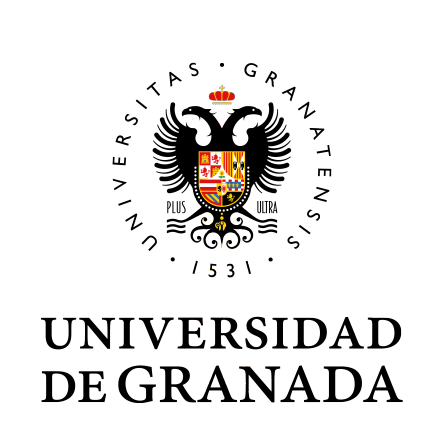
\includegraphics[scale=0.5]{img/ugr.png}\\

\includegraphics[scale=0.3]{img/logo_ugr.jpg}\\[1cm]

\textsc{\Large \asignatura{}\\[0.2cm]}
\textsc{GRADO EN INGENIERÍA INFORMÁTICA}\\[1cm]

\noindent\rule[-1ex]{\textwidth}{1pt}\\[1.5ex]
\textsc{{\Huge \titulo\\[0.5ex]}}
\textsc{{\Large \subtitulo\\}}
\noindent\rule[-1ex]{\textwidth}{2pt}\\[3.5ex]

\end{minipage}

%\vspace{0.5cm}
\vspace{0.7cm}

\begin{minipage}{\textwidth}

\centering

\textbf{Autor}\\ {\autor{}}\\[2.5ex]
\textbf{Rama}\\ {\rama}\\[2.5ex]
\vspace{0.3cm}


\includegraphics[scale=0.3]{img/etsiit.jpeg}

\vspace{0.7cm}
\textsc{Escuela Técnica Superior de Ingenierías Informática y de Telecomunicación}\\
\vspace{1cm}
\textsc{Curso 2019-2020}
\end{minipage}
\end{titlepage}

\pagenumbering{arabic}
\tableofcontents
\thispagestyle{empty}				% No usar estilo en la pagina de indice

% start new page before setting page layout,
% otherwise previous page is also affected
\KOMAoption{paper}{landscape}%
\typearea{12}% sets new DIV

% Establecer pagina horizontal
\recalctypearea
% needed to show page in landscape in viewer
\pdfpageheight=\paperheight
\pdfpagewidth=\paperwidth
% Poner estilo
\pagestyle{lscape}


\setlength{\parskip}{1em}

\section{Diagrama de clases}

\begin{figure}[H]
  \centering
  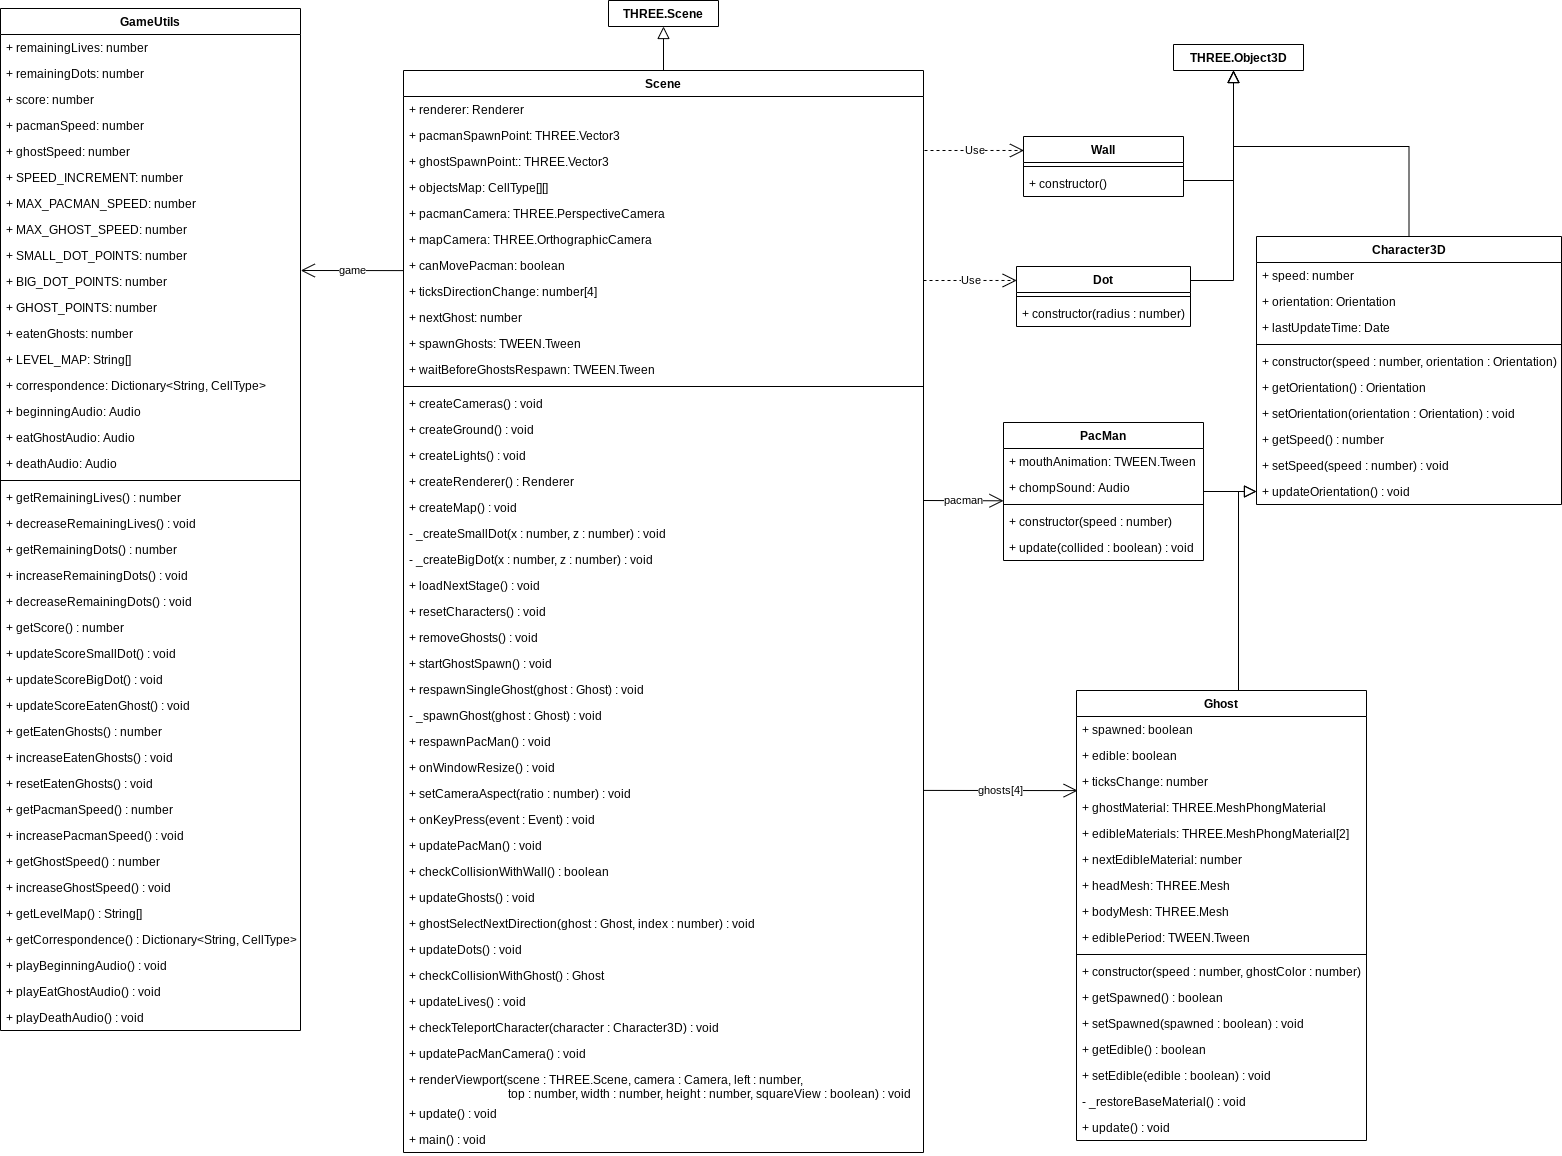
\includegraphics[scale=0.365]{img/diagrama-clases}
\end{figure}

\KOMAoptions{paper=portrait}
\recalctypearea
\pdfpageheight=\paperheight
\pdfpagewidth=\paperwidth
\headwidth\textwidth

Partiendo del diagrama de clases anterior, vamos a describir las clases para que se entienda
qué representa cada una de ellas.

\subsection{Clase \texttt{Character3D}}

Esta clase representa un personaje 3D, heredando de la clase \texttt{THREE.Object3D}. El personaje
tiene un atributo \texttt{speed}, que se refiere a la velocidad a la que se mueve por segundo;
un atributo \texttt{orientation}, que indica hacia donde está orientado el personaje (arriba,
abajo, izquierda o derecha); y un atributo que indica el tiempo en el que se realizó la última
actualización del personaje, es decir, en qué momento se llamó por última vez al método
\texttt{update()} de la clase correspondiente. De esta forma se puede conseguir que los
personajes se muevan de forma independiente a la cantidad de fotogramas que sea capaz de
renderizar el ordenador, tal y como se ha estudiado en clase.

El método más destacable es \texttt{updateOrientation()}. Este método se llama desde el método
\texttt{update()} de las clases derivadas y se encarga de rotar al personaje de manera que mire en
la dirección que le indique el atributo \texttt{orientation}.

\subsection{Clase \texttt{PacMan}}

Esta clase representa al personaje \texttt{Pac-Man}. Hereda de la clase \texttt{Character3D},
con lo cuál hereda sus métodos y atributos. Tiene dos atributos, que son \texttt{mouthAnimation}
y \texttt{chompSound}. El primero es la animación de la boca, la cuál consiste en rotar dos
semiesferas en el eje Z cada una en un sentido. Cuando ambas llegan al final del movimiento,
comienzan a realizarlo en sentido contrario. Dicho movimiento se repite indefinidamente,
deteniéndose solamente cuando el personaje colisiona con un muro. El otro atributo es el sonido
del personaje al moverse. Dicho sonido se reproduce siempre y cuando el personaje se esté
moviendo, es decir, que no haya colisionado con un muro.

El método \texttt{update()} recibe un parámetro, el cuál indica si el personaje ha colisionado
contra un muro (verdadero) o no (falso). En caso de que valga verdadero no se actualiza la
posición del personaje , se detiene la animación de la boca si no estaba ya detenida y se pausa
el sonido del movimiento. En caso contrario, se actualiza la posición en función de la
orientación del personaje, se reproduce el sonido y se actualiza la animación de \texttt{Tween},
continuando con esta o reanudándola en función de si estaba pausada o no anteriormente.

\subsection{Clase \texttt{Ghost}}

Esta clase representa a un fantasma del juego. Hereda de la clase \texttt{Character3D},
con lo cuál hereda sus métodos y atributos. En este caso merece la pena comentar casi todos
los atributos propios, ya que tienen una importancia significativa:

\begin{itemize}
	\item El atributo \texttt{spawned} es un booleano que indica si el fantasma ha aparecido en
	el escenario o no.
	\item El atributo \texttt{edible} indica si el fantasma es comestible o no.
	\item \texttt{ticksChange} es un atributo que se utiliza en la animación que se
	lanza cuando el fantasma es comestible. Básicamente, una vez que haya pasado el 70\%
	del tiempo de la animación, cada 100 \textit{ticks} o actualizaciones de la animación
	el material del fantasma va a ir cambiando, dando la sensación de intermitencia. El material
	va a ir cambiando entre el azul oscuro y el blanco.
	\item \texttt{ghostMaterial} es el material base del fantasma.
	\item El atributo \texttt{edibleMaterials} es un \textit{array} que contiene los 
	dos materiales que tiene el fantasma mientras puede ser comido: el azul oscuro y el blanco.
	\item El atributo \texttt{nextEdibleMaterial} es el índice del siguiente material que se
	va a utilizar en la animación. Empieza con el valor 0, refiriéndose por tanto al azul
	oscuro, y después se incrementa para hacer referencia al blanco. Después va cambiando de
	valor cada 100 \textit{ticks} como se ha explicado anteriormente.
	\item \texttt{bodyMesh} y \texttt{headMesh} son los \textit{mesh} que forman el cuerpo
	y la cabeza del fantasma, respectivamente. Es necesario guardarlos, ya que el material
	de estos se va a ver modificado cuando el fantasma pasa a ser comestible y cuando deja
	de serlo.
	\item Por último, \texttt{edibleMaterial} es la animación que controla el momento en el
	que el fantasma es comestible. Tiene una duración de 8 segundos y se activa cuando el
	\texttt{Pac-Man} se come un punto grande. Puede terminar antes de los 8 segundos si el
	jugador se come al fantasma. Una vez que se acaba, el fantasma deja de ser comestible.
\end{itemize}

La clase tiene un par de \textit{setters} y \textit{getters}, además del método
\texttt{update()}, el cuál se encarga de controlar el movimiento del fantasma en función de
la orientación. No obstante, de todos ellos destacan dos. Uno de ellos es
\texttt{setEdible(edible)} el cuál cambia el valor del atributo \texttt{edible} e inicia o
detiene la animación \texttt{ediblePeriod} en función de dicho valor, además de establecer el
material del fantasma al correspondiente y de inicializar otros valores, como por ejemplo
\texttt{nextEdibleMaterials} y \texttt{ticksChange}. El otro es \texttt{\_restoreBaseMaterial()},
el cuál, como su propio nombre indica, restaura el material base del fantasma. Este es un
método auxiliar utilizado por el anterior y por la animación una vez que esta haya sido
completada.

\subsection{Clase \texttt{Wall}}

Esta clase hereda de \texttt{THREE.Object3D} y representa un muro del juego, el cuál es de color
azul oscuro. Su constructor simplemente crea una caja de tamaño $1 \times 1 \times 1$ y la
posiciona sobre el suelo.

\subsection{Clase \texttt{Dot}}

Esta clase hereda de \texttt{THREE.Object3D} y representa o bien un punto pequeño o uno grande
en función del radio que se utilice a la hora de crear un \textit{mesh}. Un punto pequeño tiene
un radio de $0.1$ unidades, mientras que uno grande tiene un radio de $0.2$ unidades.

\subsection{Clase \texttt{GameUtils}}

Esta es una clase que contiene toda la información del juego: puntuación del jugador, puntuación
que proporciona cada elemento del juego, número de fantasmas que se ha comido el jugador
mientras estos son comestibles, vidas restantes, puntos restantes en el mapa por comer,
velocidades de los personajes y sus velocidades máximas, audios que se utilizan en determinados
momentos de la partida (inicio de la partida, al comerse a un fantasma y al morir) y el mapa del
juego junto con su correspondencia a tipos de celdas.

La mayoría de sus métodos son \textit{getters}, además de tener otros métodos que le
permiten modificar algunos de los atributos. Hay unos pocos que son de especial interés, como
podría ser el caso de los métodos que incrementan la velocidad de los personajes, ya que
comprueban que no se ha superado el máximo antes. El incremento de velocidad es de $0.5$ cada
vez que se completa un nivel. La velocidad inicial del \texttt{Pac-Man} es de 3 unidades por
segundo, mientras que la de los fantasmas es de $2.5$. La velocidad máxima del \texttt{Pac-Man} es
de $5.5$ unidades por segundo, mientras que la de los fantasmas es de 5. De esta forma, el
personaje siempre es algo más rápido que los fantasmas.

Otro método interesante es el de aumentar la puntuación del jugador cuando se ha comido a un
fantasma. Recordemos que el primer fantasma proporciona 200 puntos, el segundo 400, el tercero 800
y el cuarto 1600. Para obtener estos valores se utiliza la siguiente fórmula:

\begin{equation}
score_{ghost} = 2^{eatenGhosts - 1} \times GHOST\_POINTS
\end{equation}

\noindent donde \texttt{GHOST\_POINTS} es la puntuación base de un fantasma, la cuál es de 200.
El restulado de esa expresión se suma a la puntuación del jugador.

\subsection{Clase \texttt{Scene}}

Esta clase hereda de \texttt{THREE.Scene} y es la que contiene como tal la escena del juego
con todos sus elementos: modelos, cámaras, información del juego, animaciones que controlan
ciertos estados del juego, etc. Vamos a describir algunos de los atributos que, en una primera
lectura, podrían no llegar a comprenderse:

\begin{itemize}
	\item \texttt{objectsMap} es un mapa que contiene qué tipo de celda hay en cada posición
	del escenario. Esta matriz no se modifica y es solo de lectura, ya que a partir de ella
	se generan los muros, los puntos y las posiciones de reaparición de los fantasmas y del
	\texttt{Pac-Man}. Toda esta información se lee del atributo \texttt{LEVEL\_MAP} de la
	clase \texttt{GameUtils}, utilizando en el proceso el atributo \texttt{correspondence}.

	\item \texttt{canMovePacman} indica si el jugador puede moverse o no. Este atributo vale
	falso al principio de la partida y al reaparecer ya que hay que esperar algunos segundos
	antes de poder empezar el movimiento, tal y como pasa en el juego original. Mientras valga
	falso la posición del personaje no se actualizará y su orientación no se podrá modificar.
	
	\item \texttt{ticksDirectionChange} es un \textit{array} que contiene, para cada uno
	de los cuatro fantasmas, un valor entero, el cuál indica cuántas llamadas al método
	\texttt{ghostSelectNextDirection(ghost, index)} han pasado desde la última vez que se modificó
	la orientación del $i$-ésimo fantasma. De esta forma se controla que si un fantasma ha
	cambiado de orientación recientemente debido a que se ha encontrado en una casilla que le
	permita hacerlo no se vuelva a intentar cambiar de orientación hasta que hayan pasado un
	número determinado de llamadas al método, el cuál es de 25.
	
	\item \texttt{spawnGhosts} es una animación que, al completarse, hace que aparezca un fantasma
	en la escena en la posición dada por \texttt{ghostSpawnPoint}. La animación es
	utilizada cuando todos los fantasmas tienen que aparecer en la escena, bien porque la partida
	ha empezado, porque el jugador ha perdido una vida o porque se ha completado el nivel (se han
	comido todos los puntos de la escena). Esta animación se tiene que completar un total de 4
	veces, por tanto se tiene que repetir 3 veces una vez que acabe. El atributo
	\texttt{nextGhost} está relacionado con esta animación, ya que indica el índice del próximo
	fantasma que tiene que aparecer en escena. La animación tiene una duración de 3 segundos por
	repetición, con lo cuál todos los fantasmas aparecerán en la escena al cabo de 12 segundos.
	
	\item \texttt{waitBeforeGhostsRespawn} es una animación que se ejecuta cuando el personaje
	reaparece después de morir o al pasar de nivel. Consiste en bloquear los movimientos del
	personaje durante 2 segundos y, una vez que acaba, iniciar la animación de aparición de
	fantasmas anteriormente descrita.
\end{itemize}

La clase tiene toda una serie de métodos, pero vamos a destacar algunos de ellos:

\begin{itemize}
	\item \texttt{createCameras()} crea las cámaras \texttt{pacmanCamera}, una cámara en
	perspectiva que sigue la posición del \texttt{Pac-Man}, y \texttt{mapCamera}, una cámara
	con vista ortográfica sobre el escenario, de forma que este se pueda ver desde el aire.
	
	\item \texttt{startGhostSpawn()} es el método encargado de gestionar la animación
	\texttt{spawnGhosts}, iniciándola y haciendo que se repita el número de veces necesario.
	
	\item \texttt{loadNextStage()} carga el siguiente nivel, volivendo a poner todos los
	puntos sobre el mapa y reseteando todos los personajes. La posición original de los puntos
	se encuentra en la matriz \texttt{objectsMap}.
	
	\item \texttt{resetCharacters()} es el método encargado de resetear a todos los personajes
	bien porque el jugador ha perdido una vida o bien porque se ha completado el nivel.
	
	\item \texttt{removeGhosts()} elimina a los fantasmas de la escena y restablece sus
	valores a los iniciales.
	
	\item \texttt{respawnSingleGhost(ghost)} hace reaparecer a un único fantasma cuando este
	es comido por el jugador.
	
	\item \texttt{\_spawnGhost(ghost)} es un método auxiliar utilizado para hacer aparecer a un
	fantasma.
	
	\item \texttt{respawnPacMan()} permite hacer reaparecer al \texttt{Pac-Man} cuando este
	ha muerto o ha pasado de fase. La forma de hacerlo es eliminando al que ya había en la
	escena y creando de nuevo al personaje, de forma que tanto su orientación como la animación
	de la boca se reinicien a los valores por defecto.
	
	\item \texttt{checkCollisionWithWall()} es el método responsable de comprobar si el
	jugador va a colisionar con un muro o no.
	
	\item \texttt{ghostSelectNextDirection(ghost, index)} es el método encargado de
	elegir la siguiente orientación del fantasma \texttt{ghost}, el cuál se encuentra en la
	posición \texttt{index} del \textit{array} de fantasmas. Para ello, se tienen que haber
	hecho más de 25 llamadas a este método para dicho fantasma, además de que no puede
	estar en cualquiera de los extremos de la fila central, ya que estos conectan la parte
	izquierda del mapa con la derecha y viceversa. Teniendo la posición del fantasma, la cuál
	ha sido truncada para que se pueda consultar la matriz, se comprueban las casillas
	contiguas (la casilla de arriba, la de abajao, la de la izquierda y la de la derecha de
	la actual). Si alguna de estas está libre y se da que la posición de dicha casilla es
	perpendicular a la orientación actual del fantasma, se puede cambiar de orientación (por
	ejemplo, si el fantasma se mueve hacia abajo y resulta que la casilla a su izquierda
	está libre). Se miran entonces cuáles son las nuevas potenciales orientaciones que puede
	tomar el fantasma con la condición de que la nueva orientación no puede ser la contraria a
	la actual (por ejemplo, si estaba orientado hacia abajo, la nueva orientación no puede ser
	arriba), evitando de esta forma que los fantasmas vuelvan sobre sus pasos. De entre las
	posibles orientaciones se selecciona una de forma aleatoria, y si resulta que la nueva
	orientación es distinta a la anterior, se reondea la posición del fantasma, ya que se ha
	producido un giro y es necesario ajustar dicha posición para que no parezca que atraviesa
	las paredes.
	
	\item \texttt{updateDots()} comprueba si el \texttt{Pac-Man} ha entrado en contacto con
	alguno de los puntos y realiza las acciones correspondientes.
	
	\item \texttt{checkCollisionWithGhost()} comprueba si el jugador ha colisionado con
	alguno de los fantasmas y devuevle el primer fantasma con el que ha colisionado.
	
	\item \texttt{checkTeleportCharacter(character)} comprueba si el personaje \texttt{character},
	el cuál puede ser o bien el jugador o bien alguno de los fantasmas, 	se encuentra en la fila
	central del mapa y en alguno de los extremos, lo cuál le permitiría 	cambiar su posición de
	un extremo al otro. En caso afirmativo, modifica su posición.
	
	\item El método \texttt{renderViewport(...)} se ha extraído de las transparencias, ya que
	se necesitan mostrar dos cámaras a la vez: la cámara en perspectiva que sigue al jugador
	y la ortográfica, la cuál proporciona una visión del mapa desde el aire. La única diferencia
	es el parámetro \texttt{squareView}, el cuál indica si el \textit{viewport} tiene que ser
	cuadrado o no (el del mini mapa es cuadrado, por ejemplo).
\end{itemize}

Es importante destacar una cosa respecto al movimiento tanto del jugador como de los fantasmas.
Ya que no se han utilizado librerías de físicas ni de colisiones, al girar podría darse el caso
de que un personaje atravesase los muros. Para evitar esto, si la nueva orientación del
personaje es perpendicular a la que tenía anteriormente se redonde la posición de dicho
personaje, de forma que al moverse en la nueva dirección no se atraviese ningún muro. 

\section{Interacción entre elementos de la escena}

Para la interacción entre los elementos de la escena no se ha utilizado ninguna librería de
físicas ni que permita detectar colisiones. Todas las colisiones e interacciones se han hecho
a mano. En esta sección se darán algunas pequeñas pinceladas de cómo se han hecho. Si se quiere
ver la implementación para obtener información más detallada, se recomienda mirar los métodos
correspondientes en la clase \texttt{Scene}.

\subsection{Interacción entre el \texttt{Pac-Man} y los muros}

La interacción básica entre el \texttt{Pac-Man} y los muros es la colisión. Dicha colisión
se comprueba, tal y como se ha dicho en la sección anterior, en el método
\texttt{checkCollisionWithWall()}. Para hacerlo basta con obtener la posición
del \texttt{Pac-Man} en $X$ y $Z$ y truncarlas. Tras hacer muchas pruebas, se ha visto
que esta es la mejor forma de determinar si el personaje colisiona o no con un muro, ya que
en caso de colisión se consigue detener el movimiento justo en la casilla en frente de este.
Una vez que se han obtenido dichas posiciones basta consultar, en función de la orientación del
personaje, si la casilla siguiente es o no un muro, lo cuál indica si va a colisionar o no
si sigue moviéndose en esa dirección.

\subsection{Interacción entre el \texttt{Pac-Man} y los puntos}

Al moverse por el mapa, el \texttt{Pac-Man} colisiona con los puntos, y estos le ofrecen
una puntuación, y en caso de ser un punto grande, hace que los fantasmas sean comestibles.
Para detectar la colisión con estos se utiliza el método \texttt{updateDots()}. Lo primero que se
hace es obtener la posición en los ejes $X$ y $Z$ del personaje, se les suma $0.5$ y se trunca
dicho valor. Se ha comprobado que haciendo estas operaciones los puntos desaparecen cuando el
personaje pasa por encima de ellos en vez de hacerlo antes o después.

Una vez obtenidas las coordenadas, hay que determinar si hay o no un punto en dicha posición.
Los puntos como tal no tienen una referencia dentro de la clase que permita acceder rápidamente
a ellos. Por eso, a la hora de crearlos se les ha asignado un nombre, el cuál permitirá buscarlos
dentro del grafo de escena. Los puntos pequeños tienen el nombre
$smallDot\_X\_Z$ y los grandes $bigDot\_X\_Z$, siendo $X$ la coordenada en el eje $X$ y
$Z$ la coordenada en el eje $Z$. Entonces, simplemente basta con buscar si hay algún punto
pequeño o grande en dicha posición mediante el nombre. En caso de haber alguno se hacen
las acciones correspondientes y se elimina dicho punto de la escena.

\subsection{Interacción entre el \texttt{Pac-Man} y los fantasmas}

La interacción entre los fantasmas y el \texttt{Pac-Man} es la colisión. En función de si el
fantasma con el que colisiona es comestible o no se hace una cosa u otra. La función encargada
de comprobar si existe colisión es \texttt{checkCollisionWithGhost()}, tal y como se mencionó
previamente.

Para comprobar si existe colisión se obtiene la posición del \texttt{Pac-Man} de la misma forma
que se hace a la hora de comprobar si colisiona con algún punto. Después, para cada uno
de los fantasmas que esté vivo (es decir, que su atributo \texttt{spawned} sea verdadero) se
obtiene su posición de la misma forma que la del \texttt{Pac-Man} y se comprueba si ambas
coinciden, en cuyo caso habría una colisión. Si exite alguna colisión, se devuelve una referencia
al primer fantasma con el que colisiona el \texttt{Pac-Man}, y en caso contrario, se devuelve
\texttt{undefined}, indicando que no se ha colisionado con ningún fantasma.

\section{Material extra utilizado}

Todas las pistas de audio se han extraído de la siguiente página:
\url{https://www.classicgaming.cc/classics/pac-man/sounds}

El icono del \texttt{Pac-Man} utilizado tanto para representar las vidas restantes como
de icono de la página se puede descargar de la siguiente página:
\url{https://www.freepng.es/png-nuufwd/download.html}

\end{document}

